\documentclass{article}\usepackage[]{graphicx}\usepackage[]{xcolor}
% maxwidth is the original width if it is less than linewidth
% otherwise use linewidth (to make sure the graphics do not exceed the margin)
\makeatletter
\def\maxwidth{ %
  \ifdim\Gin@nat@width>\linewidth
    \linewidth
  \else
    \Gin@nat@width
  \fi
}
\makeatother

\definecolor{fgcolor}{rgb}{0.345, 0.345, 0.345}
\newcommand{\hlnum}[1]{\textcolor[rgb]{0.686,0.059,0.569}{#1}}%
\newcommand{\hlstr}[1]{\textcolor[rgb]{0.192,0.494,0.8}{#1}}%
\newcommand{\hlcom}[1]{\textcolor[rgb]{0.678,0.584,0.686}{\textit{#1}}}%
\newcommand{\hlopt}[1]{\textcolor[rgb]{0,0,0}{#1}}%
\newcommand{\hlstd}[1]{\textcolor[rgb]{0.345,0.345,0.345}{#1}}%
\newcommand{\hlkwa}[1]{\textcolor[rgb]{0.161,0.373,0.58}{\textbf{#1}}}%
\newcommand{\hlkwb}[1]{\textcolor[rgb]{0.69,0.353,0.396}{#1}}%
\newcommand{\hlkwc}[1]{\textcolor[rgb]{0.333,0.667,0.333}{#1}}%
\newcommand{\hlkwd}[1]{\textcolor[rgb]{0.737,0.353,0.396}{\textbf{#1}}}%
\let\hlipl\hlkwb

\usepackage{framed}
\makeatletter
\newenvironment{kframe}{%
 \def\at@end@of@kframe{}%
 \ifinner\ifhmode%
  \def\at@end@of@kframe{\end{minipage}}%
  \begin{minipage}{\columnwidth}%
 \fi\fi%
 \def\FrameCommand##1{\hskip\@totalleftmargin \hskip-\fboxsep
 \colorbox{shadecolor}{##1}\hskip-\fboxsep
     % There is no \\@totalrightmargin, so:
     \hskip-\linewidth \hskip-\@totalleftmargin \hskip\columnwidth}%
 \MakeFramed {\advance\hsize-\width
   \@totalleftmargin\z@ \linewidth\hsize
   \@setminipage}}%
 {\par\unskip\endMakeFramed%
 \at@end@of@kframe}
\makeatother

\definecolor{shadecolor}{rgb}{.97, .97, .97}
\definecolor{messagecolor}{rgb}{0, 0, 0}
\definecolor{warningcolor}{rgb}{1, 0, 1}
\definecolor{errorcolor}{rgb}{1, 0, 0}
\newenvironment{knitrout}{}{} % an empty environment to be redefined in TeX

\usepackage{alltt}
\IfFileExists{upquote.sty}{\usepackage{upquote}}{}
\begin{document}





\section*{Showcase real-world examples of time series visualisations.}

Time series of the daily CNY, CAN, EUR, HKD, USD versus GBP exchange reference rate data
published by the European Central Bank over the time period from 01 Jan 2013 to 12 Oct 2023 (without weekends). The exchange rate tells you how many pounds you need to buy/sell 1 CNY, CAN, EUR, HKD, USD.

\subsection{The data set has the format as below:}

\begin{table}[h]
\centering
\begin{tabular}{|c|c|c|c|c|c|}
\hline
\textbf{Date} & \textbf{CNYtoGBP} & \textbf{CANtoGBP} & \textbf{EURtoGBP} & \textbf{HKDtoGBP} & \textbf{USDtoGBP} \\
\hline
\%d-\%m-\%y & Value & Value & Value & Value & Value \\
\hline
& & & & & \\
\hline
\end{tabular}
\caption{Field Information: CNY, CAN, EUR, HKD, USD to GBP}
\end{table}


\subsection{Multiple time series in one plot:}

\begin{knitrout}
\definecolor{shadecolor}{rgb}{0.969, 0.969, 0.969}\color{fgcolor}
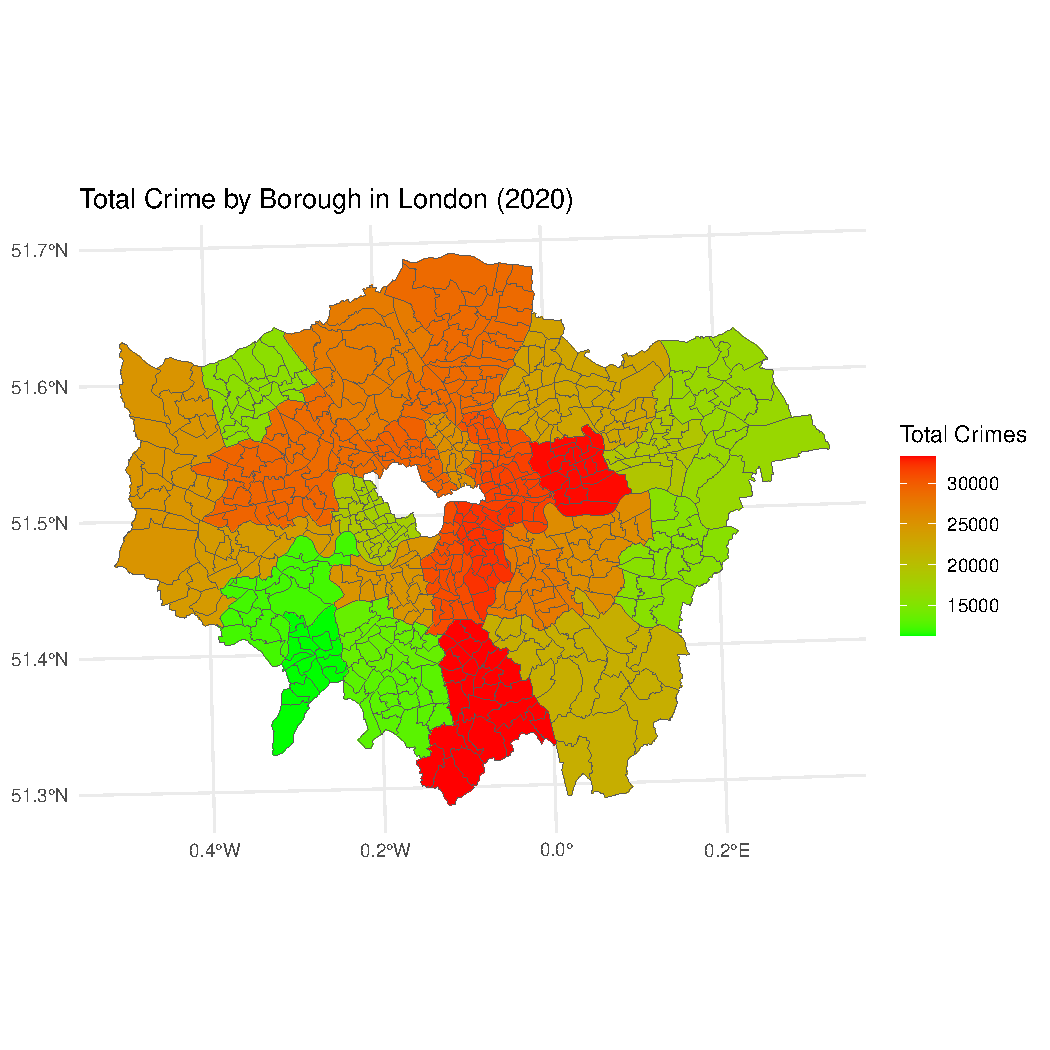
\includegraphics[width=\maxwidth]{figure/unnamed-chunk-1-1} 
\end{knitrout}


\begin{knitrout}
\definecolor{shadecolor}{rgb}{0.969, 0.969, 0.969}\color{fgcolor}\begin{kframe}
\begin{alltt}
\hlcom{# Calculate 21-day moving average for each currency}
\hlstd{columns} \hlkwb{<-} \hlkwd{names}\hlstd{(MyData)[}\hlopt{!}\hlkwd{names}\hlstd{(MyData)} \hlopt \hlstr{"Date"}\hlstd{]}
\hlkwa{for} \hlstd{(col} \hlkwa{in} \hlstd{columns) \{}
  \hlstd{new_col_name} \hlkwb{<-} \hlkwd{paste0}\hlstd{(col,} \hlstr{"_MA7"}\hlstd{)}
  \hlstd{MyData[[new_col_name]]} \hlkwb{<-} \hlstd{zoo}\hlopt{::}\hlkwd{rollapply}\hlstd{(MyData[[col]],} \hlkwc{width}\hlstd{=}\hlnum{21}\hlstd{,} \hlkwc{FUN}\hlstd{=mean,} \hlkwc{fill}\hlstd{=}\hlnum{NA}\hlstd{,} \hlkwc{align}\hlstd{=}\hlstr{'right'}\hlstd{)}
\hlstd{\}}

\hlcom{# Plotting}
\hlstd{plot_data} \hlkwb{<-} \hlstd{MyData} \hlopt \hlkwd{gather}\hlstd{(}\hlkwc{key}\hlstd{=}\hlstr{"Currency"}\hlstd{,} \hlkwc{value}\hlstd{=}\hlstr{"Rate"}\hlstd{,} \hlopt{-}\hlstd{Date)} \hlopt
  \hlkwd{filter}\hlstd{(}\hlkwd{grepl}\hlstd{(}\hlstr{"MA7"}\hlstd{, Currency))}

\hlkwd{ggplot}\hlstd{(plot_data,} \hlkwd{aes}\hlstd{(}\hlkwc{x}\hlstd{=Date,} \hlkwc{y}\hlstd{=Rate,} \hlkwc{color}\hlstd{=Currency))} \hlopt{+}
  \hlkwd{geom_line}\hlstd{()} \hlopt{+}
  \hlkwd{labs}\hlstd{(}\hlkwc{title}\hlstd{=}\hlstr{"7-Day Moving Average of Exchange Rates"}\hlstd{,}
       \hlkwc{subtitle}\hlstd{=}\hlstr{""}\hlstd{,}
       \hlkwc{y}\hlstd{=}\hlstr{"Exchange Rate to GBP (21-Day MA)"}\hlstd{,}
       \hlkwc{x}\hlstd{=}\hlstr{"Date"}\hlstd{,}
       \hlkwc{color}\hlstd{=}\hlstr{"Currency"}\hlstd{)} \hlopt{+}
  \hlkwd{theme_minimal}\hlstd{()} \hlopt{+}
  \hlkwd{scale_color_brewer}\hlstd{(}\hlkwc{palette}\hlstd{=}\hlstr{"Set1"}\hlstd{)}
\end{alltt}


{\ttfamily\noindent\color{warningcolor}{\#\# Warning: Removed 100 rows containing missing values (`geom\_line()`).}}\end{kframe}
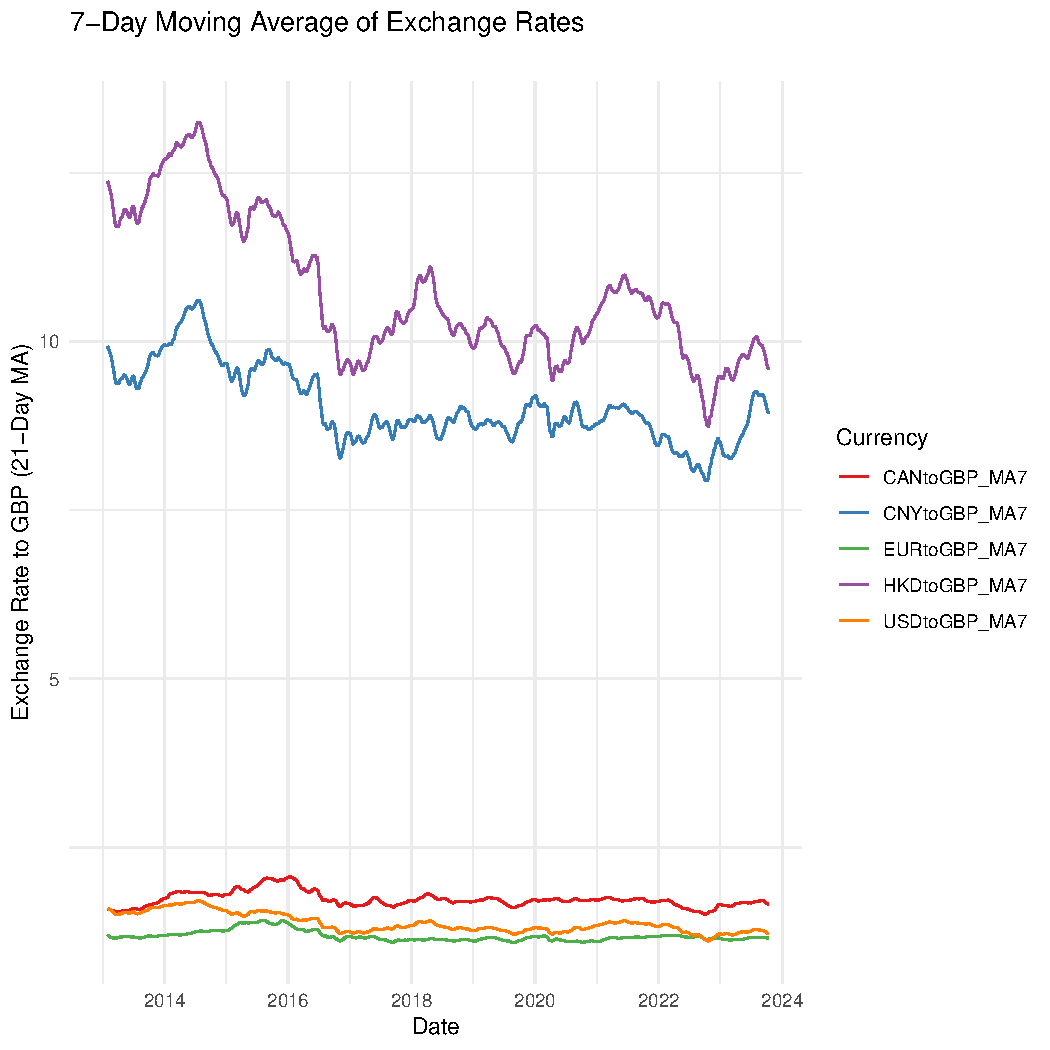
\includegraphics[width=\maxwidth]{figure/unnamed-chunk-2-1} 
\end{knitrout}




\subsection{Decomposition of one time series into trend, seasonal, and random.}


One of the primary advantages of time series visualization is the ease with which it allows analysts to identify long-term upward or downward trends in data and patterns that repeat over specific intervals. By decomposing the time series, it would be easy to see those features.

\begin{knitrout}
\definecolor{shadecolor}{rgb}{0.969, 0.969, 0.969}\color{fgcolor}
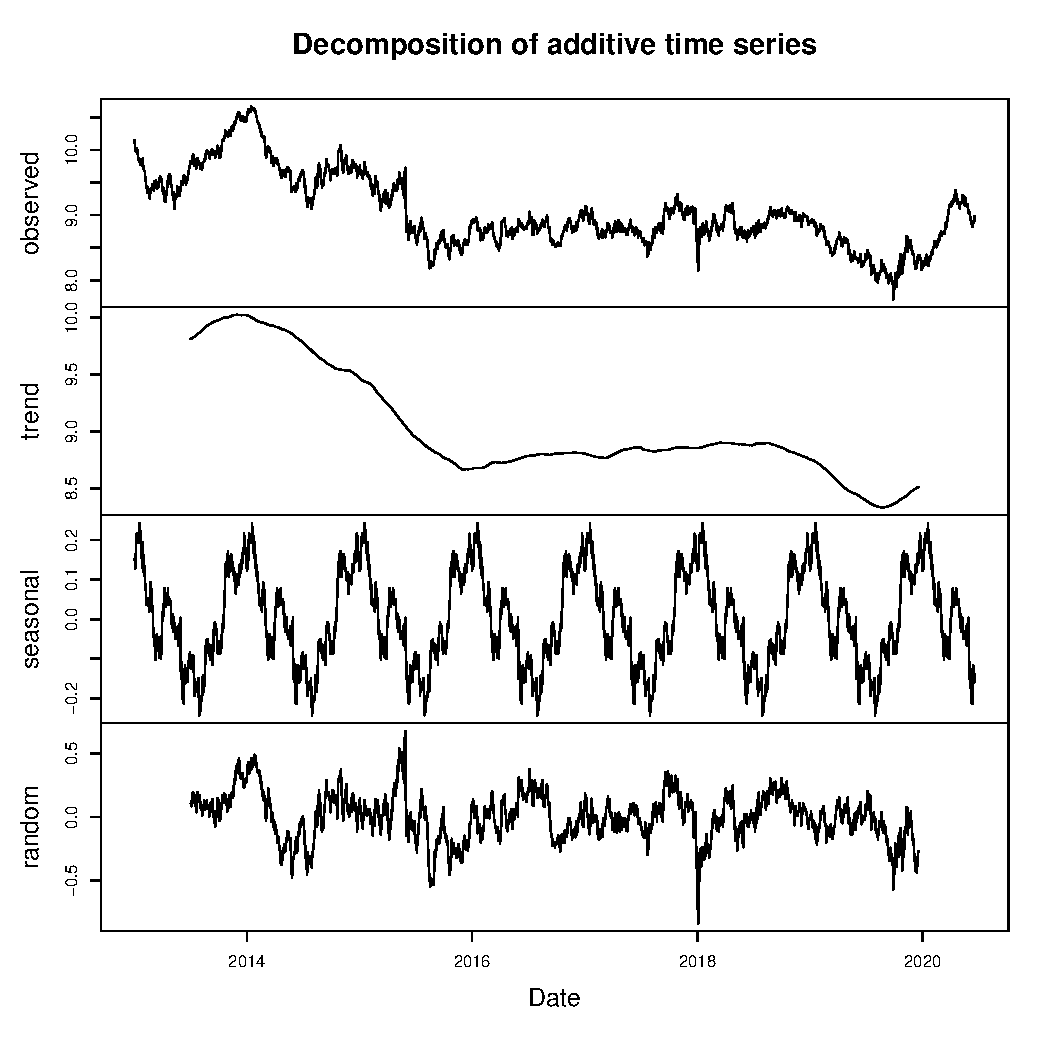
\includegraphics[width=\maxwidth]{figure/unnamed-chunk-3-1} 
\end{knitrout}





\subsection{Cyclical plots}

For data with clear cyclical patterns (e.g., daily, weekly, monthly), plotting data in a circular fashion can highlight these cycles.

\begin{knitrout}
\definecolor{shadecolor}{rgb}{0.969, 0.969, 0.969}\color{fgcolor}\begin{kframe}
\begin{alltt}
\hlstd{MyData}\hlopt{$}\hlstd{Month} \hlkwb{<-} \hlkwd{month}\hlstd{(MyData}\hlopt{$}\hlstd{Date,} \hlkwc{label} \hlstd{=} \hlnum{TRUE}\hlstd{)}
\hlstd{MyData}\hlopt{$}\hlstd{Day} \hlkwb{<-} \hlkwd{day}\hlstd{(MyData}\hlopt{$}\hlstd{Date)}

\hlkwd{ggplot}\hlstd{(MyData,} \hlkwd{aes}\hlstd{(}\hlkwc{x} \hlstd{= Month,} \hlkwc{y} \hlstd{= USDtoGBP))} \hlopt{+}
  \hlkwd{geom_path}\hlstd{(}\hlkwd{aes}\hlstd{(}\hlkwc{group} \hlstd{= Day),} \hlkwc{color} \hlstd{=} \hlstr{"blue"}\hlstd{)} \hlopt{+}
  \hlkwd{coord_polar}\hlstd{(}\hlkwc{start} \hlstd{=} \hlnum{0}\hlstd{)} \hlopt{+}
  \hlkwd{labs}\hlstd{(}\hlkwc{title} \hlstd{=} \hlstr{"Cyclical Plot of USD to GBP"}\hlstd{)} \hlopt{+}
  \hlkwd{theme_minimal}\hlstd{()}
\end{alltt}
\end{kframe}
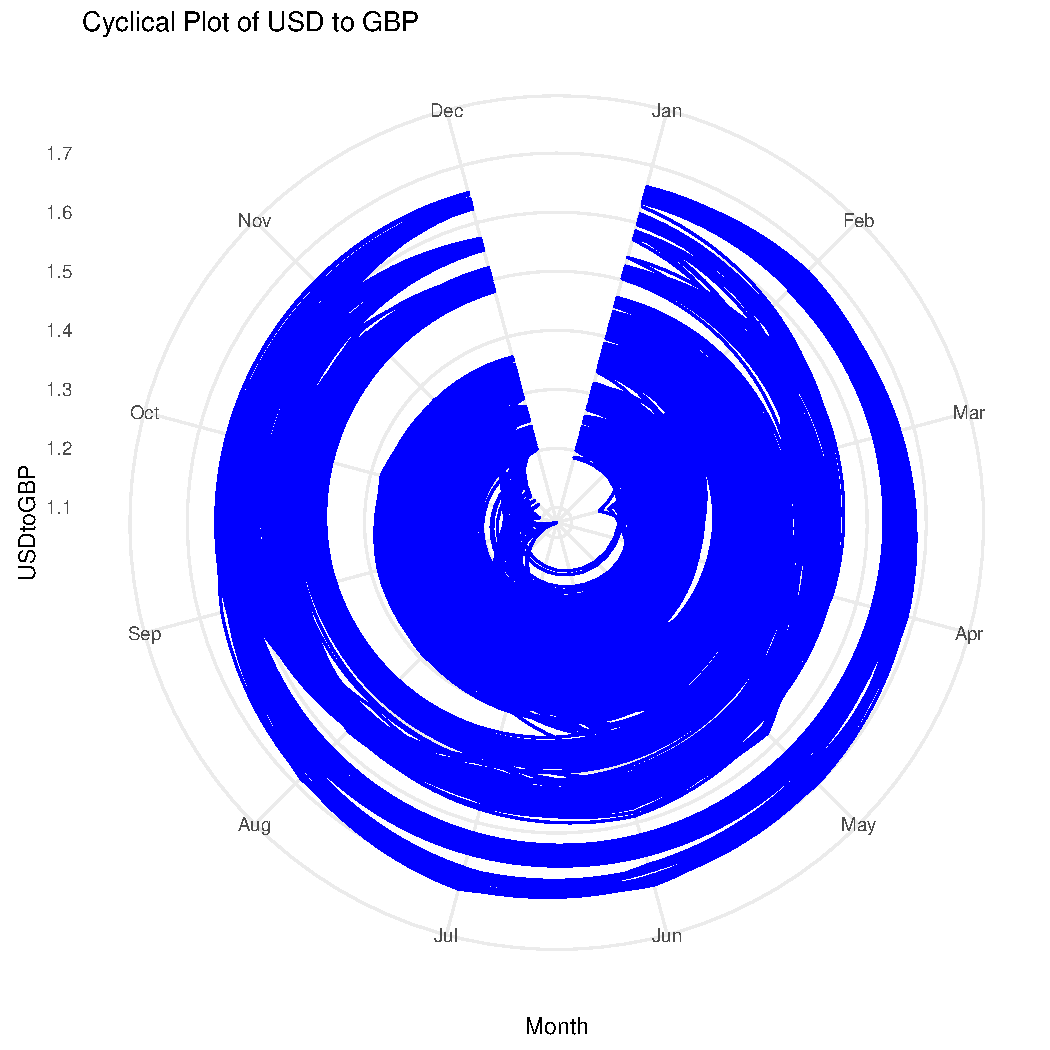
\includegraphics[width=\maxwidth]{figure/unnamed-chunk-4-1} 
\end{knitrout}















\subsection{Animated Time Series:}
This type of visualization allows for the observation of changes over time in an animated fashion. plotly is a great library for this.
\begin{knitrout}
\definecolor{shadecolor}{rgb}{0.969, 0.969, 0.969}\color{fgcolor}\begin{kframe}
\begin{alltt}
\hlstd{selected_columns} \hlkwb{<-} \hlkwd{c}\hlstd{(}\hlstr{"CNYtoGBP"}\hlstd{,} \hlstr{"EURtoGBP"}\hlstd{)}

\hlcom{# Create an interactive line chart}
\hlstd{plot_data} \hlkwb{<-} \hlstd{MyData} \hlopt
  \hlkwd{select}\hlstd{(Date,} \hlkwd{all_of}\hlstd{(selected_columns))} \hlopt
  \hlkwd{gather}\hlstd{(}\hlkwc{key}\hlstd{=}\hlstr{"Currency"}\hlstd{,} \hlkwc{value}\hlstd{=}\hlstr{"Rate"}\hlstd{,} \hlopt{-}\hlstd{Date)}

\hlstd{fig} \hlkwb{<-} \hlkwd{plot_ly}\hlstd{(}\hlkwc{data} \hlstd{= plot_data)} \hlopt
  \hlkwd{add_trace}\hlstd{(}\hlkwc{x} \hlstd{=} \hlopt{~}\hlstd{Date,} \hlkwc{y} \hlstd{=} \hlopt{~}\hlstd{Rate,} \hlkwc{color} \hlstd{=} \hlopt{~}\hlstd{Currency,} \hlkwc{type}\hlstd{=}\hlstr{"scatter"}\hlstd{,} \hlkwc{mode}\hlstd{=}\hlstr{"lines"}\hlstd{)} \hlopt
  \hlkwd{layout}\hlstd{(}\hlkwc{title} \hlstd{=} \hlstr{"Interactive Exchange Rates Over Time"}\hlstd{,}
         \hlkwc{xaxis} \hlstd{=} \hlkwd{list}\hlstd{(}\hlkwc{title} \hlstd{=} \hlstr{"Date"}\hlstd{),}
         \hlkwc{yaxis} \hlstd{=} \hlkwd{list}\hlstd{(}\hlkwc{title} \hlstd{=} \hlstr{"Exchange Rate to GBP"}\hlstd{),}
         \hlkwc{hovermode} \hlstd{=} \hlstr{"x"}\hlstd{)}

\hlcom{# Display the plot}
\hlstd{fig}
\end{alltt}


{\ttfamily\noindent\color{warningcolor}{\#\# Warning in RColorBrewer::brewer.pal(N, "{}Set2"{}): minimal value for n is 3, returning requested palette with 3 different levels}}

{\ttfamily\noindent\color{warningcolor}{\#\# Warning in RColorBrewer::brewer.pal(N, "{}Set2"{}): minimal value for n is 3, returning requested palette with 3 different levels}}

{\ttfamily\noindent\bfseries\color{errorcolor}{\#\# Error in loadNamespace(name): there is no package called 'webshot'}}\end{kframe}
\end{knitrout}



\subsection{Double y-axis time series plot.}

If we want to display two different time series that measure two different quantities at the same time points, we can draw the second series again on the second Y-axis on the right side.

\begin{knitrout}
\definecolor{shadecolor}{rgb}{0.969, 0.969, 0.969}\color{fgcolor}
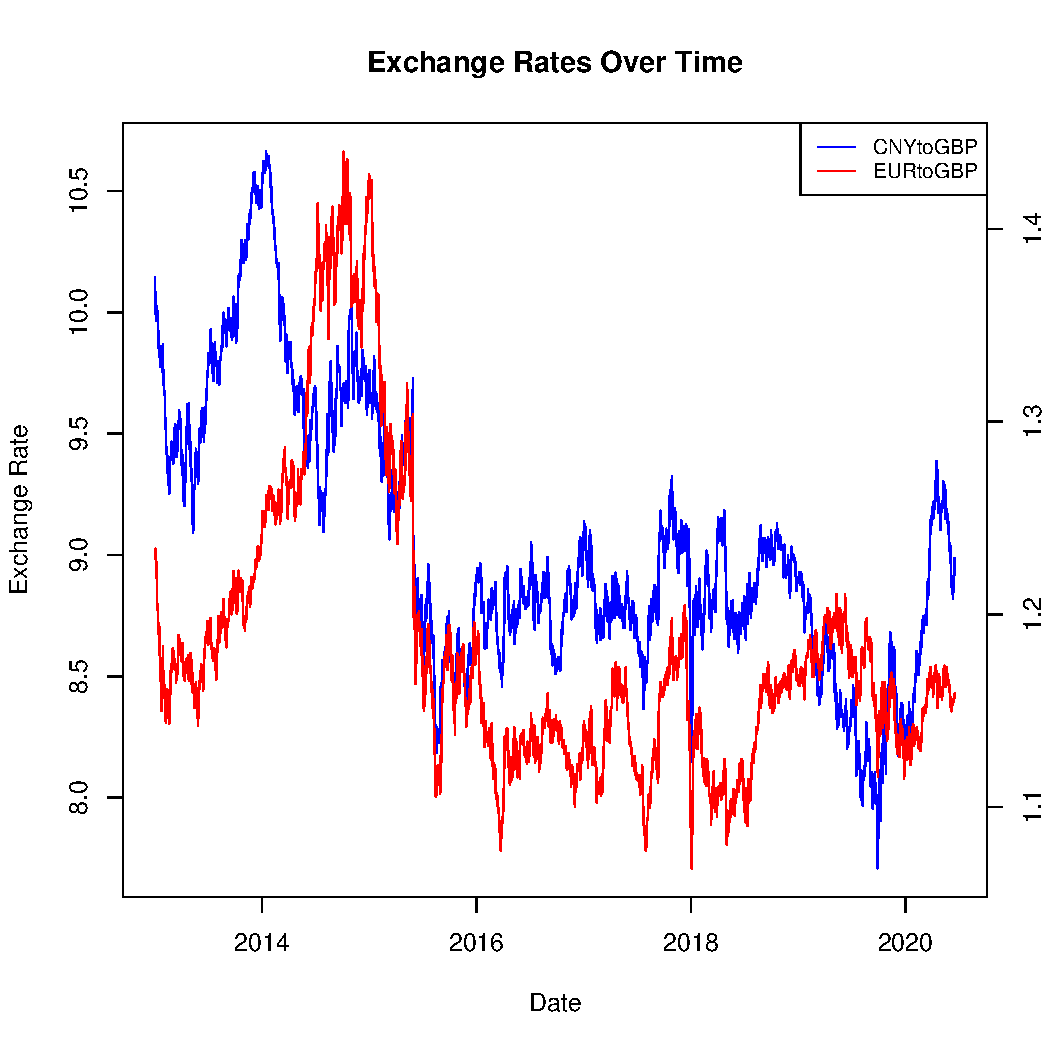
\includegraphics[width=\maxwidth]{figure/unnamed-chunk-6-1} 
\end{knitrout}


\end{document}
